\documentclass[a4paper,10pt]{article}
\usepackage{geometry}
\usepackage{mathtools}
\usepackage{amsfonts}
\usepackage{amsmath}

\usepackage[utf8]{inputenc}

 \geometry{
 a4paper,
 total={170mm,257mm},
 left=20mm,
 top=30mm,
 }
\usepackage{fancyhdr}
\fancyhead[L]{Leonard Korp 302582 \\ Nikita Malyschkin 319500 \\ Valentin Engelke 358096}
\fancyhead[R]{WS 2017/18 \\ 2.11.2017}
\pagestyle{fancy}



\begin{document}
\centerline{\Large\bfseries  Foundations of Data Science }
\centerline{\bfseries  Exercise sheet 5}
\section*{Exercise 1}
\subsection*{a)}
The following proof uses  $\ln x \leq x-1 \ \forall x$\\
\begin{align*}
&D(q||p) \\
&= (-1) \sum\limits_{i=1}^n q_i \ln \frac{p_i}{q_i} \\
&\geq (-1) \sum\limits_{i=1}^n q_i  (\frac{p_i}{q_i}-1)\\
&= (-1) \sum\limits_{i=1}^n p_i-q_i\\
&= \sum\limits_{i=1}^n q_i - \sum\limits_{i=1}^n p_i\\
&=0
\end{align*}


\section*{Exercise 2}
\subsection*{a)}
\[f(d,k)= 2^{d-k} {{d}\choose{k}}\]
\subsection*{b)}
\[\sum_{k=0}^d 2^{d-k} {{d}\choose{k}} =\sum_{k=0}^d 2^{d-k} 1^k {{d}\choose{k}}= (2+1)^d=3^d \]
This follows from the binomial theorem. 
\subsection*{c)}
The surface area of a d dimensional unit cube is the number of d-1 dimensional faces times the area of these faces. 
\[A=f(d,d-1)*1^{d-1}=2^1 {{d} \choose {d-1}}= 2 \frac{d!}{(d-1)!1!}=2d\] 
\subsection*{d)}
\[A=f(d,d-1)*2^{d-1}=2^1 {{d} \choose {d-1}}*2^{d-1}= 2 \frac{d!}{(d-1)!1!}*2^{d-1}=2d*2^{d-1}\]
\section*{Exercise 3}
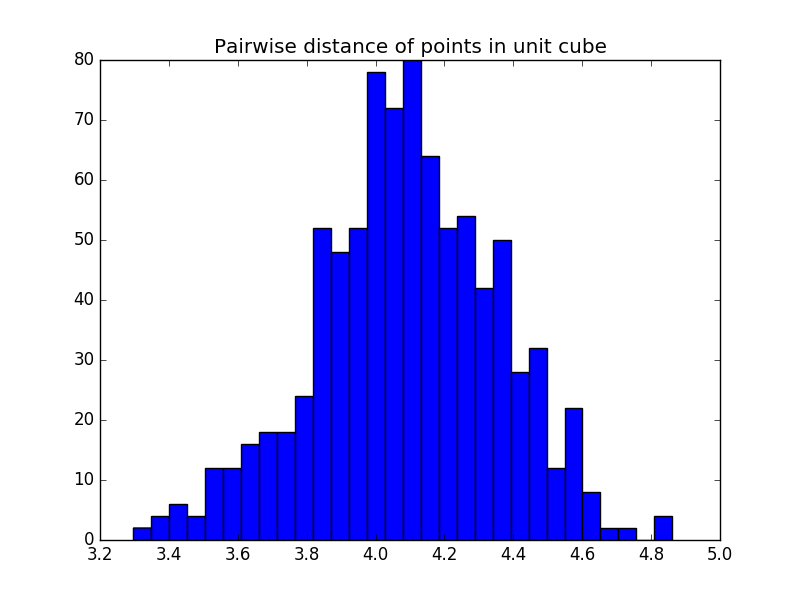
\includegraphics[scale=.4]{c_dist}
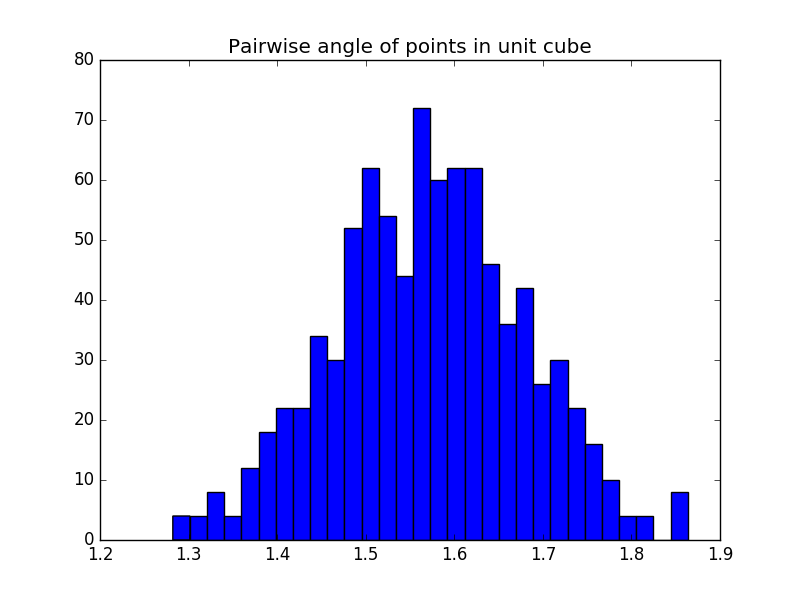
\includegraphics[scale=.4]{c_angle}

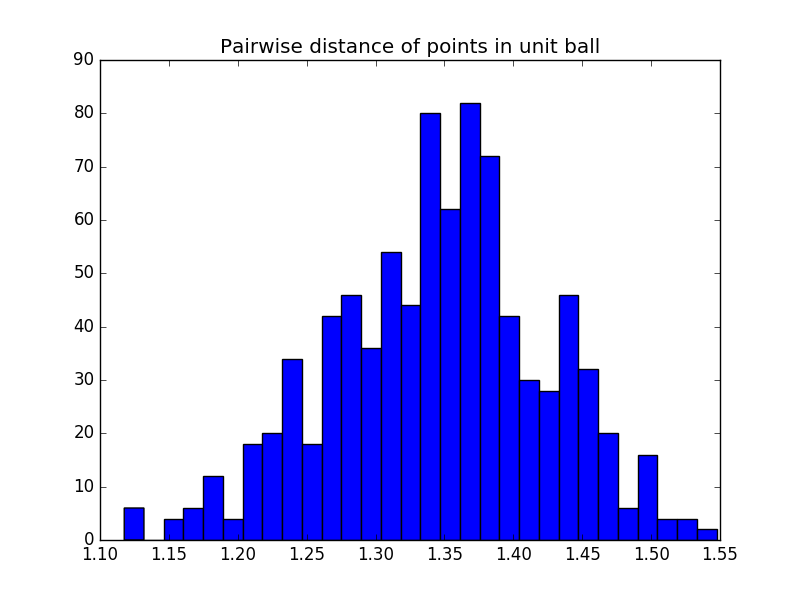
\includegraphics[scale=.4]{b_dist}
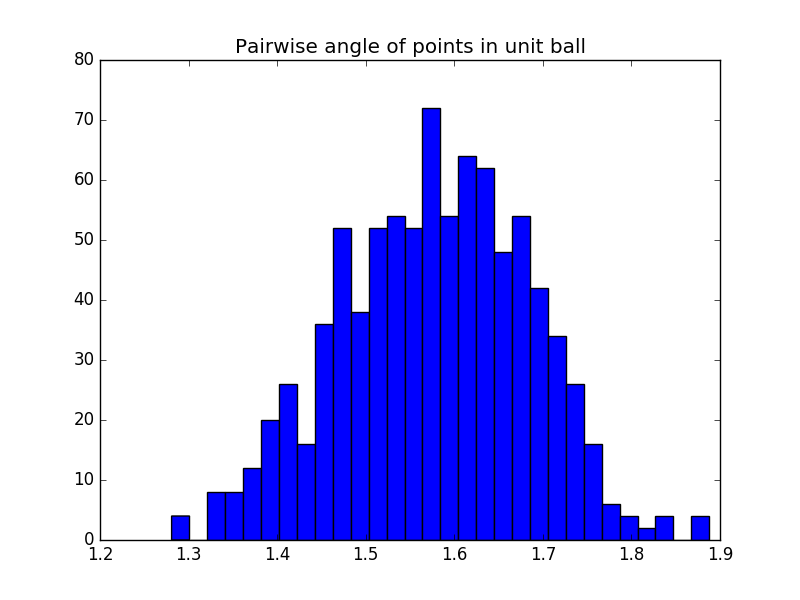
\includegraphics[scale=.4]{b_angle}
\end{document}

